\chapter{Referencial Teórico}\label{cap:referencial_teorico}

\section{Mineração de opinião}\label{sec:mineracao_dados}

É de conhecimento comum que há um acúmulo de dados por toda a internet. Artigos, informações de usuários, comportamento de usuários, são alguns tipos de informação que podem ser encontrados hoje na internet. Esse grande acúmulo não garante informações confiáveis ou uma análise correta sobre os dados, por isso há uma grande urgência para novas teorias computacionais e ferramentas que ajudem a avaliar essa quantidade de dados gerados \cite{fayyad1996data}. E dentro dessa enorme gama de dados, existem as informações adicionadas por usuários através de texto, que remetem a suas reações a determinadas situações ou objetos.

\begin{figure}[H]
	\centering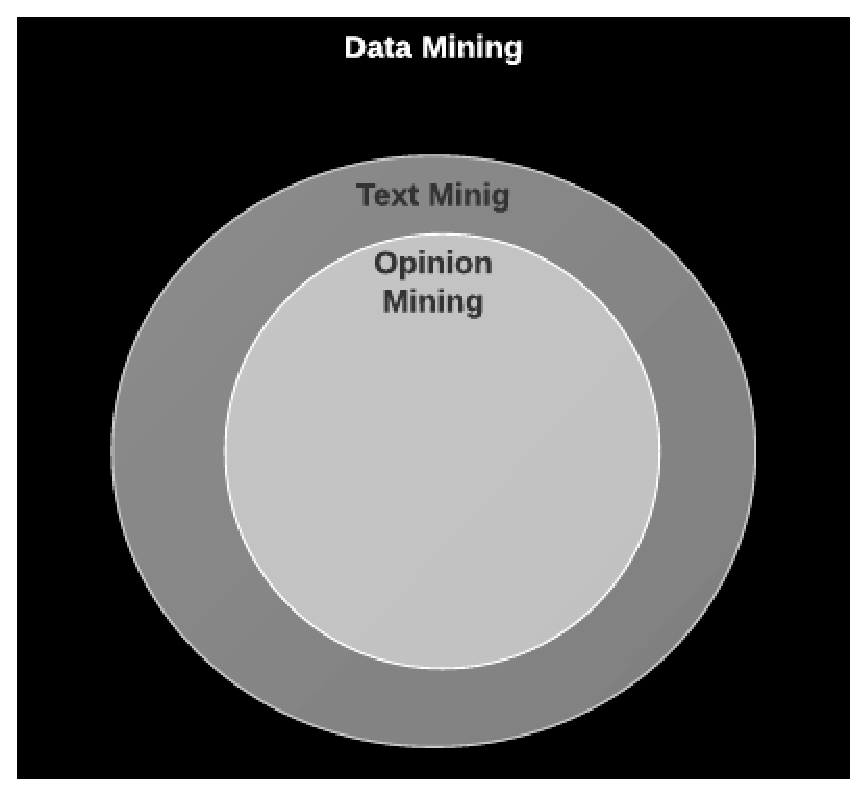
\epsfig{file=figuras/venn.eps, width=15cm}
	\caption{Visualizando as sete áreas práticas de mineração de texto e algumas de suas tarefas. \cite{miner2012practical} }
	\label{venn}
\end{figure}

De acordo com a figura \ref{venn}, o presente trabalho atua em uma área de interseção entre o processamento de linguagem natural, classificação de documento e extração de conceito.

\subsection{Sentimento}
De acordo com psicólogo Klaus R. Scherer, sentimento é um breve episódio da resposta sincronizada de todos os ou grande parte dos subsistemas orgânicos em resposta a um evento interno ou externo de grande significância\cite{scherer2001emotional}. Algumas outras definições utilizadas são:
\begin{itemize}
	\item Ato ou efeito de sentir;
	\item Aptidão para receber as impressões;
	\item Sensação, sensibilidade;
	\item Consciência íntima;
	\item Faculdade de compreender, intuição e percepção.
\end{itemize}

A mineração de opinião, também conhecida como mineração de sentimento, análise de sentimento ou extração de opinião, é um campo dentro da mineração de dados \cite{santos2014mineraccao} que tem como objetivo extrair o sentimento do texto escrito por uma pessoa, sem a interferência humana durante o processo.

\subsection{Desafios}

No campo de mineração de opinião, existem uma série de desafios que devem ser tidos como grandes pontos de atenção para quem deseja aplicar essa técnica de forma correta. 

\begin{itemize}
	\item Em blogs e redes sociais é comum encontrar textos com erros de ortografia ou escritos de forma informal, contendo gírias e abreviações comuns dentro da comunicação virtual;
	\item Dificuldade em discernir uma opinião ou um fato, especialmente quando existem opiniões embutidas em fatos;
	\item Os textos podem conter ironias e sarcarmos, que são especialmente difíceis de serem identificados e podem impactar os resultados;
	\item Um texto pode se referir à dois temas diferentes - política e ideologia, por exemplo - com opiniões diferentes sobre os mesmos, o que pode confundir a classificação;
\end{itemize}

\subsection{Etapas}

O processo de mineração de opinião consiste em 3 etapas: \cite{mineracaoopiniaoufsc}

\begin{itemize}
	\item Coleta de dados;
	\item Classificação;
	\item Análise dos resultados;
\end{itemize}

\subsubsection{Coleta de dados}

Nesta etapa é conduzida uma busca por opiniões nas mais diversas fontes que podem ser úteis: artigos, sites, comentários, anúncios, dentre outras. Como explicado anteriormente, deve-se visar identificar se a informação coletada é uma opinião ou fato. Fatos podem ser descartados imediatamente, porém opiniões apresentadas através de fatos, podem ser úteis.

Existem diversas maneiras de coletar sistematicamente fontes para extrair e armazenar os dados que serão utilizados, dentre elas as mais famosas estão o desenvolvimento \textit{crawlers} - uma rotina sistemática capaz de varrer sites em busca de informações - e a utilização de APIs.

\subsubsection{Classificação}

A classificação é a alma do processo de mineração de opinião. Nesta etapa é determinada a polaridade do objeto de estudo em positivo, negativo e neutro.

Essa etapa é a principal responsável pela acurácia da análise. Por ser a etapa mais delicada do processo é onde ocorrem a maior parte dos erros. Existem diversas técnicas e ferramentas que ajudam a mitigar tais problemas que serão abordadas mais adiante, no Capítulo~\ref{cap:proposta}.

\subsubsection{Análise dos resultados}

A análise dos resultados envolve cruzar as informações de polaridade obtidas através texto com qualquer outra informação que exista sobre quem produziu aquela opinião. Desta forma, é possível, por exemplo, determinar qual gênero - masculino ou feminino - tem uma maior aceitação à um produto ou personalidade. As possibilidades para cruzar os dados e obter \textit{insights} será proporcional a quantidade de informações coletadas durante o processo.

\subsection{Aplicações práticas}

Um algoritmo capaz de extrair opiniões de um texto pode ser aplicado em diversos cenários:

\subsubsection{Pesquisa de opinião sobre um produto}

Mineração de opinião pode ser usada por uma empresa para determinar se um certo produto lançado ao mercado atingiu a aceitação prevista, como forma de entender a percepção do público e guiar estrategicamente ações de marketing e relações públicas. Ainda é possível prospectar o sentimento associado a um produto antes mesmo do seu lançamento, visando antecipar \textit{insights} que podem ser valiosos durante o seu desenvolvimento.

\subsubsection{Análise sobre pessoas públicas}

Da mesma forma, é possível utilizar a mesma técnica e direcionar as análises para uma personalidade pública. Por exemplo, é possível determinar a aceitação ou rejeição de um político durante o mandato ou período de eleições, gerando dados que podem ser decisivos na definição de suas estratégias de campanha. 

\subsubsection{Mercado financeiro}

Os números do mercado financeiro são uma consequência direta do sentimento que pessoas(investidores) possuem sobre uma empresa \cite{villela2013financcas}. A opinião extraída de especialistas e sites de notícias podem ser usados como um dos fatores decisivos para compra e venda de ativos financeiros.

\subsection{Fontes de dados}

É notório que estamos rodeados de dados dentro da Internet, porém dentro do campo de minerações de opiniões, existem algumas fontes que se destacam pela abrangência e diversidade dos dados.

\subsubsection{Mecanismos de busca}

É possível utilizar mecanismos de busca para obter opiniões sobre praticamente qualquer temática. Este método possui uma particularidade: mecanismos de busca como Google e Bing destacam certas páginas de acordo com motivos desconhecidos, o que pode influenciar os resultados obtidos. De forma geral, essa análise é apenas um reflexo do que está sendo buscado naquele momento.

Um exemplo da utilização de mecanismos de busca para mineração de opinião é o site whatdoesinternetthink.net\cite{whatdoesinternetthink}, que utiliza como base os mecanismos de busca Google e Bing para determinar a opinião sobre um tema específico ou comparar dois temas entre si.

\subsubsection{Redes sociais}

O intenso compartilhamento de informações o opiniões que vemos hoje nas redes sociais serve como uma excelente fonte de dados para a mineração de opiniões por dois motivos: diversidade e abundância. Somando-se os usuários de Facebook e Twitter por exemplo, obtemos uma amostra considerável da população mundial à disposição para pesquisas.

Para este trabalho, o Twitter foi escolhido como base para a coleta de dados, por ser uma rede social focada em opiniões de usuários e pela grande facilidade que existe em consumir os seus dados através da API pública disponibilizada pelo mesmo.

A análise de redes sociais ganhou incrível relevância nos campos de pesquisa social e comportamental\cite{wasserman1994advances} com o aumento de compartilhamento de informações dentro destes ambientes. Ao invés de analisar comportamentos individuais, atitudes e crenças, a análise de redes sociais foca sua atenção em entidades sociais ou atores interagindo entre si e como essas interações constituem uma estrutura que pode ser estudada e analisada.

Outro ponto levantado recorrentemente quando o assunto é análise de redes sociais é como ela pode ser útil para estudos de ordem micro ou macro. No nível \textit{micro}, as análises destinam-se a examinar díades, tríades ou outros pequenos sub-grupos - conjuntos de dois, três ou mais atores sociais. No nível \textit{macro}, o objeto de estudo são grandes redes de atores sociais.
Todos os dados obtidos durante a coleta permitem segmentar os atores sociais de diversas formas - gênero, idade, religião, posição demográfica, entre outros. Por exemplo, os dados extraídos a partir da API do Twitter, tema abordada no Capítulo 3, nos permite entender como um usuário específico reagiu a uma \textit{hashtag}. Da mesma forma, podemos olhar um cenário mais amplo, como por exemplo, todos usuários de uma região do país. As possibilidades de análise crescem e se tornam mais ricas conforme obtemos mais informações sobre os atores no momento de suas interações sociais.

\section{Twitter}\label{sec:twitter}

Contando com uma base ativa de usuários que ultrapassa 300 milhões \cite{twittercompany2016}, o Twitter é conhecido como um \emph{microblog} fundado em março de 2006 por Jack Dorsey, Evan Williams e Biz Stone. Os usuários trocam mensagens de até 140 caracteres \cite{twittercharlimit2016} em um ambiente de rede social, que tem como objetivo dar à todos o poder de compartilhar ideias e informações instantaneamente \cite{twittercompany2016}. Após 10 anos de mercado, a empresa acumula números impressionantes: 300 bilhões de mensagens já foram compartilhadas por seus usuários, que em média enviam 500 milhões de \emph{tweets} \cite{twitterstats2016} - nome pelo qual as mensagens compartilhadas no microblog ficaram conhecidas na Internet - por dia.

Dentro do Twitter, O usuário pode fazer uso de \emph{hashtags} - marcadores conhecidos do público de rede social, que servem como uma indexação para um tópico específico \cite{waite2012paperback}. Apesar de simples, as \emph{hashtags} pode ser usadas das mais diversas maneiras:
\begin{itemize}
\item Agrupar comentários e pensamentos acerca de um tema
\item Estabelecer uma conexão entre dois tópicos
\item Aproximar o usuários de um conteúdo relevante com auxílio de uma busca
\end{itemize}

\subsection{Primavera Árabe}
Um dos exemplos mais recentes e impressionantes de como as redes sociais desempenharam o papel de aproximar ideologias semelhantes e encorajar debates sociais profundos foi a Primavera Árabe - onda de manifestações e protestos que tiveram início em dezembro de 2010, tendo como cenário o Norte da África e Oriente Médio. Os principais alvos foram os regimes ditatoriais e patriarcais que há muito tempo estavam no poder \cite{howard2011opening}. Redes sociais foram amplamente utilizadas para marcar encontros, debates e manifestações, além de mostrar para o mundo o que acontecia em tempo real, através do Twitter e outras redes sociais, como o YouTube.

\begin{figure}[H]
	\centering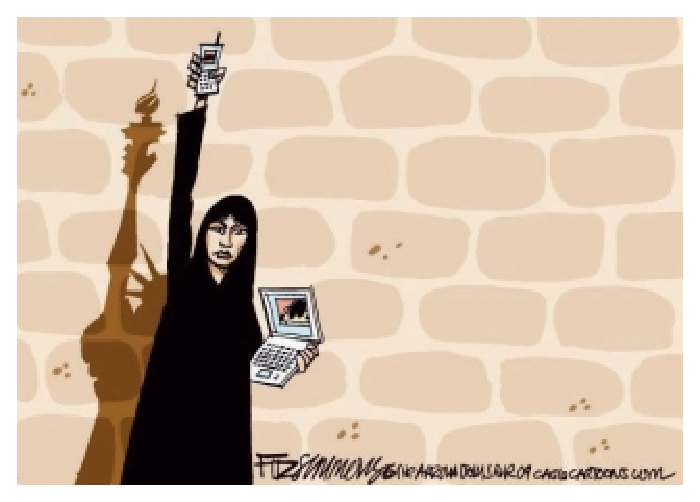
\epsfig{file=figuras/primavera_arabe_redes_sociais.eps, width=10cm}
	\caption{O celular e a internet foram as armas dos rebeldes na Primavera Árabe. Fonte: Desconhecida}
	\label{uni}
\end{figure}

\section{API}\label{sec:api}

Uma API é um conjunto de rotinas estabelecidos por um software para a utilização de suas funcionalidades e acessos aos seus dados por outro software que não pretende fazer uso de sua implementação, apenas de seus serviços. Através dessa interface, capaz de fazer uma abstração dos dados e funcionalidades de um software, conectar-se a estes serviços se torna muito mais simples.

Outro ponto que demonstra a importância das APIs durante o desenvolvimento de software é a interoperabilidade. Atualmente, temos o mesmo serviço sendo oferecido em diferentes plataformas, como por exemplo \textit{web}, \textit{desktop} e \textit{mobile}. Cada plataforma possui características e implementações diferentes, porém é possível que todas as plataformas utilizem as APIs como meio único de acesso a dados e serviços, promovendo uma padronização de protocolos e funcionalidades e serviços, além de alta reusabilidade de código.

\begin{figure}[H]
	\centering\epsfig{file=figuras/interoperabilidade_api.eps, width=10cm}
	\caption{Papel das APIs integrando dados e serviços em diferentes plataformas. Fonte: http://www.programmableweb.com/}
	\label{uni}
\end{figure}

O Twitter, possui uma API pública que pode ser utilizada por qualquer usuário da rede social \cite{twitterapidocs}. 

\begin{figure}[H]
	\centering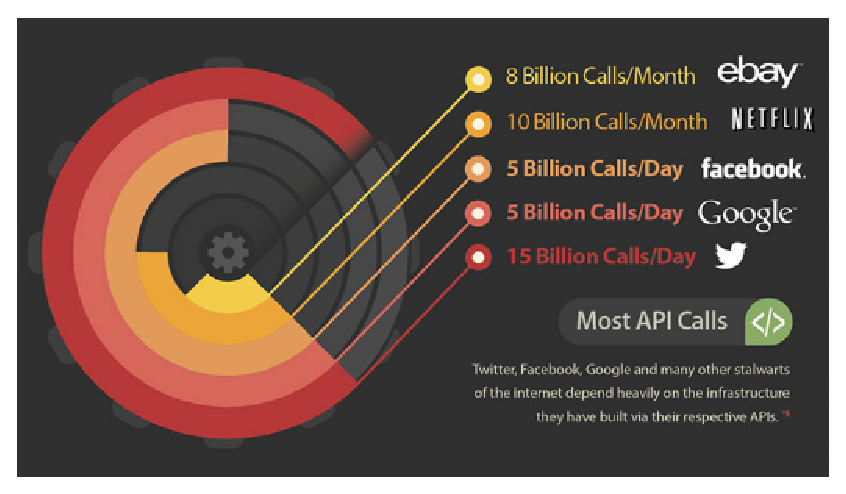
\epsfig{file=figuras/api_mais_usada.eps, width=10cm}
	\caption{APIs mais utilizadas do mundo Fonte: SmartFile}
	\label{uni}
\end{figure}

Para efetuar uma comunicação eficiente com quem acessa à API, é necessário implementar um protocolo de acesso aos dados. Os protocolos \ac{REST} e \ac{SOAP} são os mais utilizados.

\subsection{REST}
O protocolo REST foi criado em 2000 por Roy Fielding \cite{fieldingrest} como parte de sua dissertação de doutourado na \textit{University of California Irvine}. Suas principais vantagens são:

\begin{itemize}
\item Por ter sido criado dentro de um ambiente acadêmico, o objetivo do protocolo abraça a filosofia \textit{open source} - que preza por projetos onde o código é aberto a todos para manutenção e colaboração \cite{weber2004success};
\item Fácil implementação e manutenção;
\item Separa claramente a implementação do cliente e do servidor;
\item A comunicação não é controlada por uma entidade única;
\item A informação pode ser armazenada pelo cliente prevenindo múltiplas chamadas;
\item Pode retornar a informação em múltiplos formatos - \ac{JSON}, \ac{XML} , entre outros.
\end{itemize}

Por outro lado, o protocolo REST possui algumas limitações. Entre elas, podemos destacar:

\begin{itemize}
	\item Só funciona em cima do protocolo HTTP;
	\item Autorização e recursos de segurança devem ser implementados à parte.
\end{itemize}

Baseado nessas características, o protocolo REST é comumente utilizado para APIs de aplicações \textit{Web} e \textit{Mobile}, como por exemplo, as APIs do Twitter, LinkedIn e Slack.

\subsection{SOAP}
Criado em 1998 por Dave Winer et al com colaboração da Microsoft, o protocolo SOAP concentra-se em endereçar necessidades do mercado corporativo. Como vantagem, o protocolo apresenta os seguintes aspectos:

\begin{itemize}
	\item Segue uma abordagem mais formal, corporativa;
	\item Trabalha em cima de qualquer protocolo de comunicação, até mesmo assíncrono;
	\item Recursos de autorização e segurança incorporados de forma nativa;
	\item Pode ser descrito utilizando \ac{WSDL};
\end{itemize}

Entre suas principais desvantagens, pode-se citar:

\begin{itemize}
	\item Muita banda trafegando metadados;
	\item Difícil e implementação;
	\item Pouco popular entre desenvolvedores \textit{Web} e \textit{Mobile};
	\item Retorna informação apenas em XML.
\end{itemize}

Geralmente, o protocolo SOAP é mais utilizado em serviços financeiros, \textit{gateways} de pagamento e serviços de telecomunicações.

\section{Processamento de Linguagem Natural}\label{sec:pnl}

\subsection{Definição}

O \ac{PLN} baseia-se em modelos computacionais capazes de executar tarefas envolvem processar informações expresas em linguagem natural, como por exemplo, interpretação e tradução de textos. \cite{covington1994natural}.

A pesquisa na área está voltada a quatro aspectos da comunicação essenciais:

\begin{itemize}
	\item Fonologia: estudo dos sons;
	\item Morfologia: estudo da estrutura das palavras;
	\item Semântica: estudo do significado;
	\item Pragmática: estudo do significado aplicado a um contexto;
\end{itemize}

Neste trabalho, o PLN será aplicado à area da semântica e pragmática, responsável por estudar os elementos usados durante uma comunicação para se expressar através da língua (semântica) e a diversidade que pode surgir a partir de um contexto (pragmática). É também um estudo sobre como usuários de uma língua adquirem conhecimento sobre a mesma, através da comunicação oral ou escrita e como essa língua se altera ao longo do tempo.

Um dos grandes desafios da área é modelar o processamento de uma máquina para compreender uma estrutura tão complexa como uma linguagem. Existe um teste famoso na área de computação, o Teste de Turing, que levanta a questão "As máquinas podem pensar?". O teste fundamenta conceitos chave sobre a \ac{IA} , que serve como base para o PLN.

\subsection{Teste de Turing}

Introduzido pelo matemático britânico Alan Turing em seu artigo de 1950 "\textit{Computing Machinery and Intelligence} \cite{turing1950computing}, o Teste de Turing explora a capacidade de um computador demonstrar comportamento inteligente equivalente ou indistiguível dos seres humanos.

O teste é composto por três elementos: dois seres humanos, sendo um participante e um juiz e um computador.

O juiz conversa em linguagem natural com um outro ser humano e uma máquina através de um canal de texto, composto por um teclado e uma tela que apresenta a conversa. Todos os participantes estão em ambientes separados. O juiz deve ser capaz de distinguir a máquina do ser humano, caso contrário, a máquina é considerada bem sucedida no teste. O objetivo não é analisar se a máquina é capaz de responder corretamente e sim dizer quão próximas as respostas da máquina foram das do ser humano.  

\begin{figure}[H]
	\centering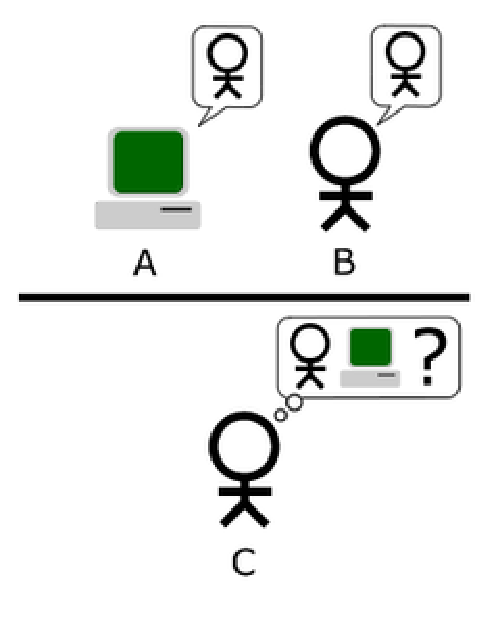
\epsfig{file=figuras/teste_turing.eps, width=10cm}
	\caption{O participante A (máquina) e o participante B (humano) se comunicam por texto com o participante C (juiz). Fonte: Wikipédia}
	\label{uni}
\end{figure}


\section{Classificador Naive Bayes}\label{sec:naive_bayes}
O classificador conhecido como \textit{Naive Bayes} é um algoritmo probabilístico baseado no Teorema de Bayes que não considera que eventuais dependências possam existir. Por este motivo, suas suposições são nomeadas ingênuas - de onde surge o nome \textit{naive} - o que lhe confere uma maior simplicidade e desempenho, em relação a outros algoritmos de classificação \cite{rennie2003tackling}. É um método popular para categorização de textos, como por exemplo a classificação de \textit{e-mails} em legítimos ou \textit{spam} - e-mails inúteis que são enviados na esperança que o receptor compre algum produto ou serviço. \cite{androutsopoulos2000evaluation}

\subsection{O Teorema de Bayes}

O Teorema de Bayes permite inferir qual é a probabilidade de um evento A dado que um evento B ocorreu e pode ser expressado pela seguinte equação:

$$ P(A \mid B) = \frac{P(B \mid A) \ P(A)}{P(B)}, $$

\begin{itemize}
	\item A e B são eventos;
	\item P(A) e P(B) são probabilidades de A e B sem considerar a relação entre ambos;
	\item P(A|B), uma probabilidade condicional, é a probabilidade de observar o evento A, dado que o evento B ocorreu.
	\item P(B|A) é a probabilidade de observar o evento B, dado que o evento A ocorreu.
\end{itemize}

Suponha que queremos saber a probabilidade de um indivíduo possuir câncer, sem saber nada sobre o indivíduo. Sabe-se que a chance de um indivíduo estar infectado com tal câncer é de 1\%, ou seja, P(A).
Em seguida, suponha que esta pessoa tenha 70 anos de idade e que essa probabilidade é de 0,2\% e que 0,5\% das pessoas doente possuem 70 anos de idade ou P(B). Se assumirmos que a incidência de câncer e a idade estão relacionadas, podemos utilizar esta informação para melhor avaliar as chances desta pessoa estar doente. Logo, queremos saber a probabilidade de uma pessoa estar doente quando a mesma possui 70 anos de idade, ou P(A|B).

$$ P(A \mid B) = (0,5\% \times 1\%) \div 0,2\% = 2,5\% $$

Portanto, o resultado do teorema demonstra que possuir 70 anos de idade aumenta a chance de uma pessoa ser portadora de câncer.

\subsection{Aplicação no trabalho}

Nese trabalho o \emph{Naive Bayes} é utilizado  para classificar \textit{tweets} em positivos, neutros ou negativos. Este algoritmo está baseado no Teorema de Bayes porém assume que a posição das palavras - eventos da probabilidade - que aparecem no texto não importa para determinar o resultado final.

Como visto em \cite{lucca2013implementaccao} o algoritmo calcula qual a probabilidade de uma frase, denominada documento pertencer a uma determinada classe(polaridade) \emph{P(C/D)}, a partir da probabilidade de \emph{P(C)} do documento pertencer a esta classe e das probabilidades condicionais de cada termo $t_{k}$ ocorrerem em um documento da mesma classe. O algoritmo tem como objetivo encontrar a melhor classe para um documento maximizando a probabilidade a posteriore. 
